\section{Brownian motion}
	\label{sec:chapter1}
	
\subsection{The Brownian motion discovery}

	
In 1827 the Scottish botanist Robert Brown published a paper \cite{robert_xxvii_1828} on his observation on the pollen of \textit{Clarkia pulchella} with a lot of details on his taught processes. His experiments was made to understand the flower reproduction, but, as he was looking through the microscope he observed some minute particles ejected from the pollen grains. At first, he thought this movement was a test to of the male organ, then looking at grains Mosses and \textit{Equiseta} which had been dried up for one hundred years, he was surprised to see this "peculiar" movement and since he was able to increase the number of particle by bruising ovula or seeds of \textit{Equisetum} he abandoned his supposition. Interestingly each time that he encountered a material that he was able to reduce to a fine enough powder to be suspended in water, he observed a constant motion, although, he never guessed the origin of the particles movement.

The difficulty at this time to observe and capture this movement made the study of what we called today Brownian motion quite difficult and the first work on erratic movement was actually done by Louis Bachelier  in 1900 in his PhD thesis "The theory of speculation", where he describe a stochastic analysis of the stock and option market. The mathematical description is still a used in the modern development of tools for the economic industry. 

It's finally in 1905 that Albert Einstein describe that "bodies of microscopically visible size suspended in a liquid will perform movements of such a magnitude that they can be easily observed in a microscope". \cite{einstein_uber_1905}. A nice remark to make here is that in 1948 Einstein wrote a letter to one of his friend where he stated having deduced the Brownian motion "from mechanics, without knowing that anyone had already observed anything of the kind" \cite{peter_brownian_nodate}.

It's in 1908 that Jean Perrin published his experimental work on the Brownian motion, that way he was able to measure the Avogadro number and prove the kinetic theory that Einstein developed. I would also cite M. Chaudesaigues and M. Dabrowski, who helped J. Perrin to track the particles by hand, half-minutes by half-minutes, for more than 3000 displacements (25 hours) and several particles. This impressive and daunting work is highly detailed in "Mouvement brownien et molécules" \cite{perrin_mouvement_1910}. This is partly due to this work than J. Perrin received the nobel award in 1926.

\begin{figure}[h]
	\centering
	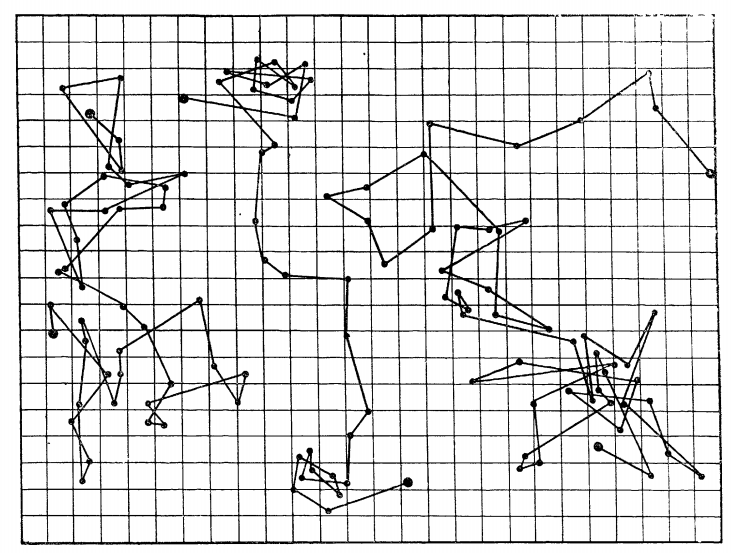
\includegraphics[scale=0.6]{02_body/chapter1/image/graph_perrin.png}
	\caption{Brownian motion of $1 ~ \mathrm{\mu m}$ particle in water tracked by hand by Jean Perrin and his colleagues, each point are timely space by 30 seconds and 16 divisions represents $50 ~ \mathrm{\mu m}$  the mean square value of was the first prove of the Einstein's kinetic theory}
	\label{fig:Perrin_Brownian}
\end{figure}

